\chapter{Przegląd problemu text-to-SQL}
Celem niniejszego rozdziału jest przedstawienie zwięzłego przeglądu problemu \code{text-to-SQL}. Najpierw wskazane zostaną popularne metryki wykorzystywane do pomiaru skuteczności tworzonych algorytmów, a następnie naszkicowane wysokopoziomowe podejścia do tego problemu, które ukształtowały się na przestrzeni lat. Zawarta wiedza stanowi podstawę do zrozumienia kolejnej części w ramach której dyskutowane i testowane będą różne modele uczenia maszynowego. 

\section{Stosowane metryki}
Posiadając docelowe zapytanie, które w literaturze anglojęzycznej określane jest mianem \code{gold query}, oraz zapytanie wyprodukowane przez dowolny algorytm zachodzi potrzeba dokonania oceny w jakim stopniu one sobie odpowiadają. Pozwala to bowiem w liczbowy sposób wyrazić dokładność algorytmu i dokonać jego porównań z innymi. Manualna ocena zwykle nie wchodzi w grę ze względu na swoją czasochłonność, więc opracowanych zostało kilka metryk, które dokonują tego w sposób automatyczny. Te najważniejsze opisano poniżej.

\subsection{Exact set match}
Problemem zwyczajnego porównywania ze sobą docelowych i przewidywanych zapytań SQL jako wartości tekstowych jest to, że mogą się one różnić w kolejności elementów nie mających znaczenia. Dla przykładu w większości przypadków nieistotnym jest w jakiej kolejności zostaną zwrócone poszczególne kolumny. Podobnie nie ma znaczenia uporządkowanie wyrażeń boolowskich połączonych operatorami \code{AND}, czy \code{OR}. Ostatecznie obojętna jest nawet kolejność występowania klauzuli \code{SELECT}, \code{FROM}, czy \code{WHERE} w strukturze zapytania. Metryka \code{exact set match} rozwiązuje naszkicowany problem poprzez odpowiednie przetworzenie zapytań i porównywanie poszczególnych składników traktując je jak zbiory, czyli ignorując kolejność, która jest tutaj nieistotna. Należy jednak zauważyć, że w języku SQL można osiągnąć ten sam cel przy pomocy kompletnie różnych instrukcji, zupełnie odmiennych strukturalnie. Metryka ta nie jest w stanie poprawnie rozpoznać takich przypadków i w rzeczywistości poprawne zapytanie oceni jako błędne.

\subsection{Exact set match without values}
Okazuje się, że szczególnie trudnym do przewidywania fragmentem zapytań SQL są wartości, czyli występujące w nich łańcuchy tekstowe i liczby. W celu oceny poprawności zapytań, lecz z dopuszczeniem różnic w tych wartościach, opracowana została metryka \code{exact set match without values}. Działa ona niemal identycznie jak \code{exact set match}, ponieważ z tą jedyną różnicą, że rozbieżności pomiędzy zapytaniami w wartościach są pomijane.

\subsection{Execution accuracy}
Metryka \code{Execution accuracy} wychodzi z prostego założenia, że jeżeli przewidziane zapytanie jest poprawne, to jego wykonanie musi zwrócić takie same rezultaty jak w przypadku zapytania referencyjnego. Ma ona jednak pewne wymagania. Przede wszystkim porównywane zapytania muszą być wykonywalne, więc zawierać wartości. Drugim warunkiem jest posiadanie wypełnionych baz danych, ponieważ w przeciwnym wypadku wszystkie zapytania będą zwracały pustą listę rekordów i tym samym zostawały błędnie uznawane za poprawne. Posiadając nawet duże bazy danych mogą zdarzyć się przypadki, iż takie same wyniki zostaną przypadkowo zwrócone dla dwóch semantycznie różnych zapytań i tym samym jedno z nich zostanie błędnie uznane za poprawne. Stanowi to podstawowe ograniczenie tej metryki.

\section{Kluczowe cechy modeli}
Dość wyraźny jest podział istniejących algorytmów rozwiązujących problem \code{text-to-SQL} ze względu na dwie cechy. Pierwsza z nich to kwestia obecności wartości w przewidywanych zapytaniach. Druga natomiast to posiadanie umiejętności wykorzystania zawartości baz danych. Informacje te w oficjalnym rankingu zbioru \code{Spider} są wyszczególnione dla każdego modelu, ponieważ mają dość istotne implikacje, które zostaną opisane w poniższych sekcjach.

\subsection{Przewidywanie wartości}
Algorytmy tłumaczące zapytania naturalne na język SQL dzielą się na dwie podstawowe kategorie: przewidujące kompletne zapytania oraz zapytania bez wartości. Wówczas produkują instrukcje zawierające w miejscu wartości specjalne symbole zastępcze, takie jak \code{value}, czy \code{terminal}. Przykłady wygenerowanych zapytań zgodnie z oboma podejściami przedstawiono na rysunku 14.

\begin{figure}[ht!]
  \centering
  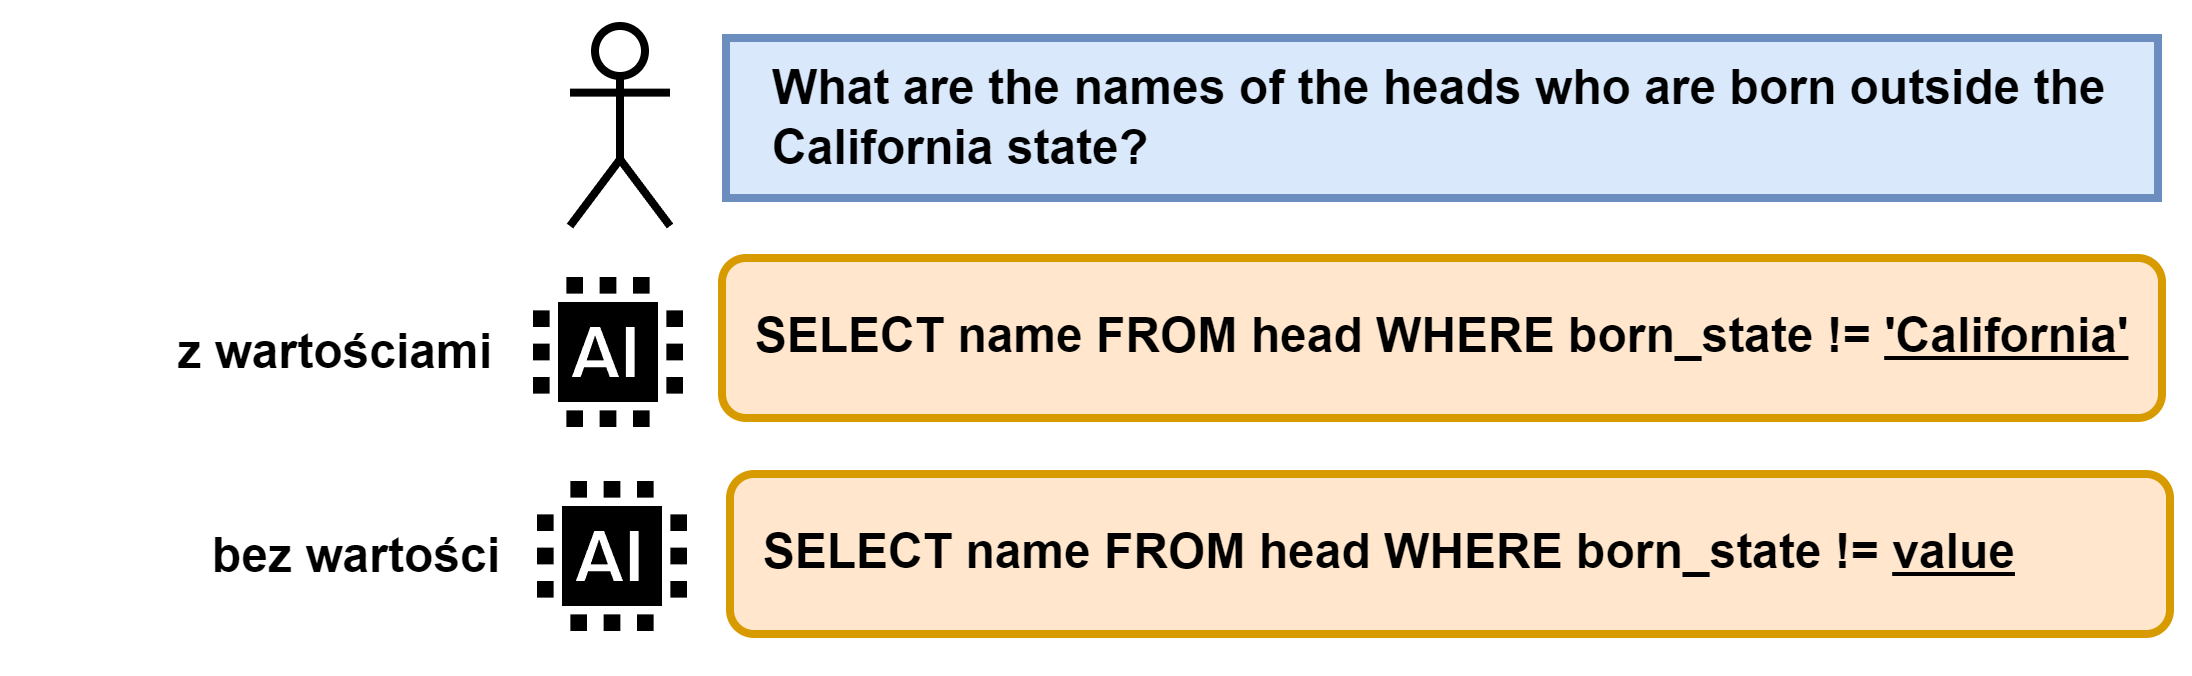
\includegraphics[width=1.0\linewidth]{images/query_values.png}
  \caption{Przykład wygenerowanego zapytania SQL z wartościami i bez}
  \label{fig:query-values}
\end{figure}

Przyczyną wyklarowania się takiego podziału jest fakt, iż wartości stanowią jeden z najtrudniejszych do wygenerowania fragmentów zapytań, a pierwsze z powstających modeli posiadały bardzo niską skuteczność. Postanowiono więc obniżyć poziom postawionego sobie zadania poprzez zignorowanie wartości i przewidywanie samej struktury zapytań. Obecnie algorytmy posunęły się jednak znacząco do przodu i osiągają wysokie wyniki nawet w generowaniu kompletnych instrukcji SQL, więc uwaga przesunęła się na ten bardziej praktyczny przypadek.

\subsection{Wykorzystanie zawartości baz danych}
Drugą istotną cechą na podstawie której można scharakteryzować wszystkie algorytmy tłumaczenia zapytań naturalnych na SQL jest to, czy korzystają one z zawartości baz danych. Podstawowym elementem na którym operują są bowiem jedynie schematy. Zawartość natomiast, pomimo, że niejednokrotnie zawiera istotne dla generowanego zapytania informacje, to wymaga zwiększenia poziomu komplikacji algorytmu. Wiąże się to także z problemem wydajnego odpytywania nieraz ogromnych zbiorów. 

Przez dłuższy czas szczyt rankingu zbioru \code{Spider} był zdominowany przez algorytmy korzystające z zawartości baz danych. Gwałtowny rozwój dużych modeli językowych umożliwił jednak poprawę dokładności nawet bez jej wykorzystania. Przewiduję się jednak, że gdy sytuacja się ustabilizuję, to branie pod uwagę zawartości baz ponownie okaże się niezbędne w celu coraz wyższego podnoszenia poprzeczki.

\section{Wysokopoziomowe podejścia}
Na obecną chwilę w rankingu \code{Spider} znajdują się modele reprezentujące dwa wysokopoziomowe, całkowicie różne od siebie podejścia. Jedno z nich polega na projektowaniu i trenowaniu modeli specjalistycznych, a drugie na wykorzystaniu dużych, pretrenowanych modeli językowych, gdzie żaden trening nie jest potrzebny. 

\subsection{Modele dedykowane}
Przez modele dedykowane, czy też specjalistyczne, rozumie się takie, które zostały stworzone w celu rozwiązania tylko jednego, konkretnego problemu. Przykładem jest tłumaczenie pytań z języka naturalnego na SQL. Takie ograniczenie pozwala na uwzględnienie i uwypuklenie w architekturze modelu oraz procesie treningu wiele istotnej dla danej domeny wiedzy. Z tego powodu możliwe jest zmniejszenie liczby potrzebnych danych i skrócenie czasu treningu. Modele tego typu dla problemu \code{text-to-SQL} istnieją od bardzo dawna i z biegiem czasu stają się coraz lepsze. W dalszej części pracy, w sekcji \ref{specific-stages}, zostało dokładniej opisane ich działanie. Jedynie w ostatnim czasie pojawiła się alternatywa w postaci dużych pretrenowanych modeli językowych.

\subsection{Duże modele językowe i prompt engineering}
Duże pretrenowane modele językowe zostały zaadaptowane w bardzo wielu problemach. Są to sieci neuronowe wytrenowane na ogromnych zbiorach danych w celu zyskania ogólnej inteligencji. Zapoczątkowało je laboratorium badawcze \code{OpenAI}, które w roku 2018 opracowało pierwszy model językowy ogólnego przeznaczenia o nazwie \code{GPT-1} \cite{Openai2018}. Szczególną uwagę całego świata zwrócił na siebie jednak dopiero model \code{GPT-3.5}, który stanowi kolejną iterację wcześniej wspomnianego. Najświeższym tego typu modelem i jednocześnie uważanym za najlepszy jest natomiast \code{GPT-4-turbo} do którego badacze mogą uzyskać dostęp za pomocą stworzonego API, by zintegrować go ze swoimi rozwiązaniami.

Wykorzystanie dużych modeli językowych opiera się na traktowaniu ich jak czarnych skrzynek, które przyjmują na wejście instrukcję w języku naturalnym i zwracają odpowiedź. Te instrukcje wejściowe mają kluczowe znaczenie i określane są mianem promptów. Nawet niewielkie ich modyfikacji mogą drastycznie wpływać na otrzymywane odpowiedzi. W związku z tym powstała cała dyscyplina określana jako \code{prompt engineering}, która zajmuję się tworzeniem oraz optymalizacją promptów w takim kierunku, aby model zwracał oczekiwane odpowiedzi.

W ostatnim czasie rozwiązania bazujące na dużych modelach językowych oraz prompt engineering zdominowały górną część rankingu zbioru \code{Spider}. Ich wadą jest jednak to, że wykorzystują płatne modele udostępniana przez \code{OpenAI}, co czyni je zbyt kosztownymi dla wielu zastosowań.

\section{Etapy tłumaczenia zapytań} \label{specific-stages}
Celem niniejszej części jest przedstawienie powszechnie występujących w dedykowanych modelach \code{text-to-SQL} etapów przetwarzania. Pozwoli to znacznie lepiej zrozumieć sposób działania rozwiązań wybranych do eksperymentów w kolejnym etapie.

Okazuje się, że niemal wszystkie powstałe do tej pory modele opierają się na architekturze \code{enkoder-dekoder}. Oznacza to, że występuje w nich etap enkodowania, podczas którego informacje wejściowe konwertowane są do zwięzłej reprezentacji pośredniej, a następnie w etapie dekodowania na jej podstawie generowana jest ostateczna odpowiedź. Etapy te mogą być jednak zrealizowane na bardzo wiele sposobów. Zwykle wyróżnia się także dodatkowy etap określany w literaturze anglojęzycznej mianem \code{schema linking}, który zwraca informację pozwalającą lepiej dokonać procesu enkodowania. 

\subsection{Schema Linking}
Celem etapu \code{schema linking} jest znalezienie powiązań pomiędzy frazami występującymi w pytaniu, a elementami bazy danych, takimi jak tabele, kolumny i wartości. Jest to działanie, które jest intuicyjnie wykonywane nawet przez ludzkich ekspertów kiedy stoją przed zadaniem skonstruowania nowego zapytania SQL. Przykładowy rezultat takiego działania przedstawiono na rysunku \ref{fig:schema-linking}. W odróżnieniu od dwóch kolejnych etapów ten jest opcjonalnych, lecz w praktyce często wykorzystywany.

\begin{figure}[ht!]
  \centering
  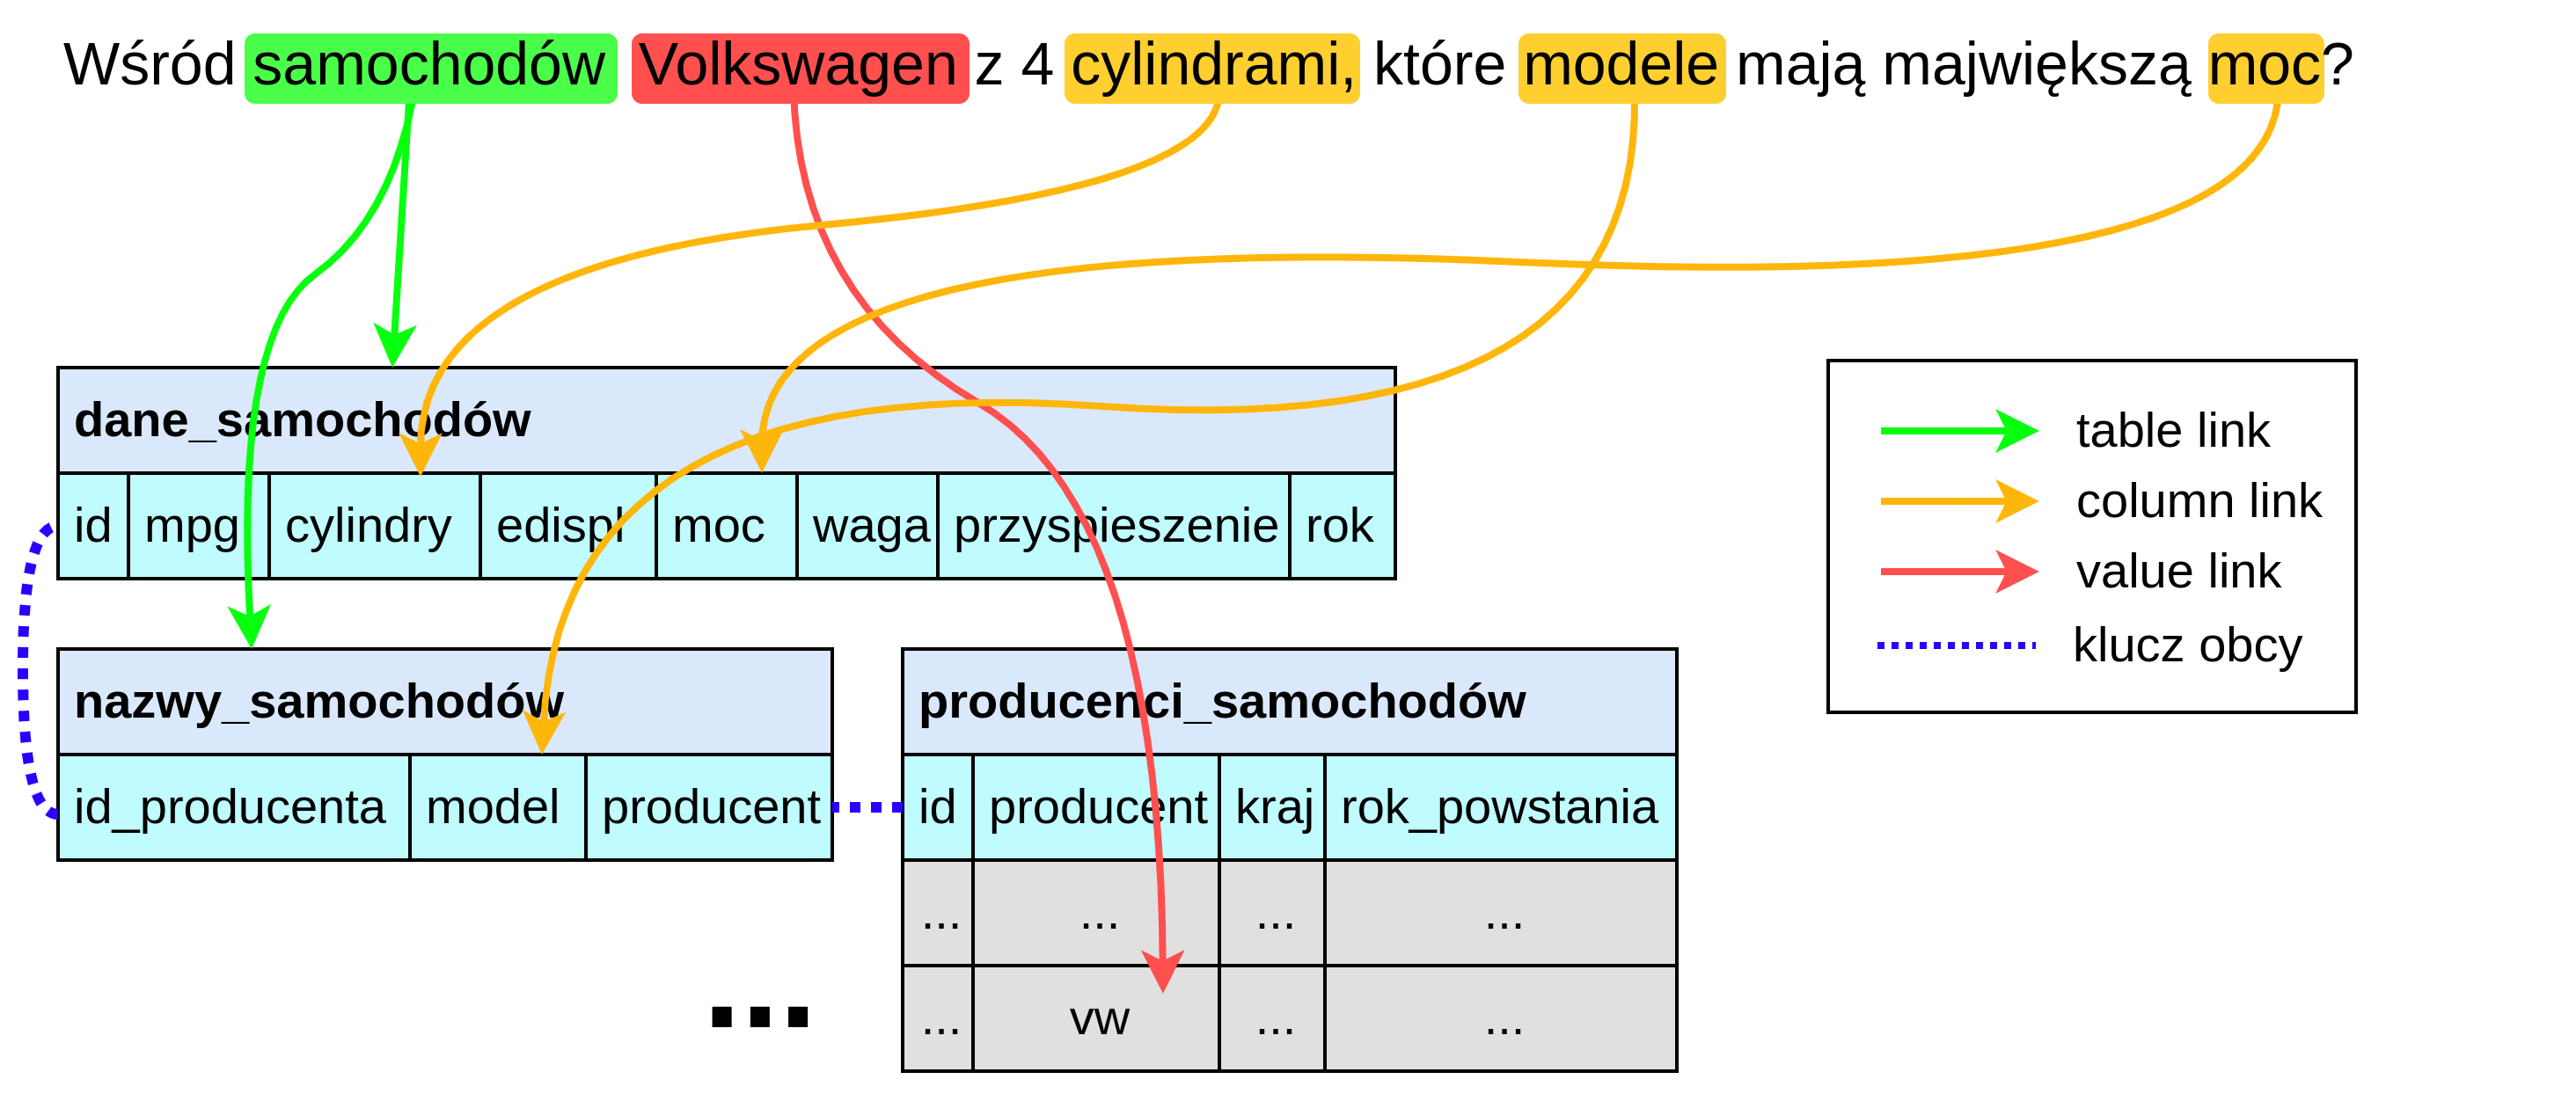
\includegraphics[width=0.8\linewidth]{images/schema_linking.png}
  \caption{Przykład wykonania \code{schema linking}}
  \label{fig:schema-linking}
\end{figure}

\code{Schema linking} można rozbić na dwie fazy. Pierwsza polega na odnalezieniu wyrażeń w pytaniach oraz elementów w bazie danych, które mogą być w kontekście budowanego zapytania istotne. Nazywane są one odpowiednio \code{query candidates} oraz \code{database candidates}. Druga faza  wymaga połączenia ze sobą tych elementów i w ten sposób skonstruowania połączeń nazywanych \code{table link}, \code{column link} lub \code{value link}, odpowiednio dla wystąpienia połączenia z tabelą, kolumną lub wartością.


Najprostsza metoda znajdywania kandydatów w pytaniu polega na uwzględnieniu każdego słowa z osobna. Wyrażenia stanowiące odwołania mogą składać się jednak z kilku słów, więc lepszym wyborem wydaje się rozważenie różnych n-gramów, czyli n-elementowych podciągów. Poza tym możliwe jest wykorzystanie analizy NER w celu znalezienia w pytaniach nazw własnych, które częstą okazują się tworzyć połączenia typu \code{value link}.

Oczywistymi kandydatami jeśli chodzi o bazę danych są wszystkie nazwy tabel i kolumn. Znacznie trudniej jest wybrać konkretne wartości, mogące tworzyć \code{value link}, bo z uwagi na ich wielość nie można brać wszystkich pod uwagę. Najczęściej dokonuję się jedynie poszukiwania w bazie konkretnych, podejrzanych wartości, które zostały ujawnione w pytaniu poprzez analizę NER, czy też zostały zapisane tam w cudzysłowach.

Po znalezieniu kandydatów zarówno w pytaniu jak i bazie danych należy spróbować dokonać ich dopasowania. Problem tutaj stanowi to, że pytania naturalne nie odwołują się najczęściej do elementów bazy poprzez dokładnie to samo określenie, lecz używają innych form i synonimów. Sprawia to, że dopasowywanie poprzez szukanie idealnych powtórzeń pomiędzy kandydatami z pytania i bazy danych często się nie sprawca, lepszą metodą jest szukanie częściowych powtórzeń. Możliwe jest też wykorzystanie odległości edycyjnej, czy odległości pomiędzy wektorowymi reprezentacjami wyrażeń.

\subsection{Enkodowanie}
Enkodowanie to etap, którego celem jest konwersja wszystkich danych wejściowych do zwartej, wektorowej postaci, czego dokonuje się za pomocą sieci neuronowej. Minimalnym zestawem informacji wejściowych jest pytanie w języku naturalnym oraz nazwy tabel i kolumn. Warte wzięcia pod uwagę są jednak także przynależności poszczególnych kolumn do tabel oraz relacje tworzone przez klucze podstawowe i obce. Jeżeli wykorzystywany został opisany wcześniej etap \code{schema linking} to znalezione podczas niego relacje również powinny w tym momencie zostać zakodowane. Poniżej opisane zostały trzy popularniejsze drogi realizacji tego etapu, lecz jest ich znacznie więcej.

Najstarsza metoda enkodowania polega na zakodowaniu pytania naturalnego oraz nazw tabel i kolumn niezależnie od siebie, a następnie połączeniu tych informacji ze sobą na którymś etapie sieci neuronowej, która jest potem trenowana. Wspomniane zakodowanie, czyli konwersja wartości tekstowych do reprezentujących je wektorów, nazywanych \code{embeddingami}, odbywa się poprzez wykorzystanie gotowych i publicznie dostępnych mapowań stworzonych z wykorzystaniem algorytmów \code{Word2Vec}, czy też \code{GloVe}.

Metodą pozwalającą osiągnąć lepsze wyniki od wcześniej wspomnianej jest serializacja informacji wejściowych do jednego długiego tekstu, który następnie jest enkodowany za pomocą pretrenowanego modelu językowego typu enkoder. Jest to zwykle model oparty na architekturze transformerów, gdzie \code{BERT} jest najczęstszym wyborem. Ich zaletą jest to, że każde słowo enkodują w sposób kontekstowy, czyli na sposób kodowania każdego słowa mają wpływ wszystkie inne. Najbardziej problematyczne w tym podejściu jest to, że nie wszystkie informacje wejściowe da się łatwo zawrzeć w czystym tekście, na przykład relacje uzyskane w wyniku \code{schema linking}, czy klucze obce.

Najbardziej elastyczną metodą, pozwalającą na wygodne zakodowanie wszystkich informacji wejściowych, jest bazowanie na reprezentacji grafowej. Wówczas poszczególne tabele, kolumny oraz słowa z pytania interpretowane są jako węzły, a znane relacje pomiędzy nimi, w tym te wydobyte na etapie \code{schema linking}, tworzą krawędzie. Czynnikiem najbardziej hamującym powszechne wykorzystanie tej strategii jest trudność związana z przetwarzaniem grafów przez sieci neuronowe. 

\subsection{Dekodowanie}
Dekodowanie to finalny etap, którego celem jest uzyskanie gotowego zapytania SQL. Bazuje na uzyskanej w fazie enkodowania reprezentacji pośredniej i również jest realizowany z wykorzystaniem sieci neuronowej. Można wskazać trzy główne nurty, w które wpisują się tworzone rozwiązania i zostaną one pokrótce opisane.

Najbardziej ograniczoną strategią jest dekodowanie oparte na szkicach (ang. sketch-based). Zakłada ono przyjęcie pewnego szablonu zapytania SQL z lukami, które należy uzupełnić. W dużej mierze sprowadza to ten etap do zadania klasyfikacji, gdyż luki wymagają często wyboru jednej z dostępnych tabel lub kolumn.  Sprawdza się to jednak wyłącznie w uproszczonych scenariuszach, na przykład zakładających wykorzystanie tylko jednej tabeli, bez żadnych połączeń. Nie ma więc wielu praktycznych zastosowań i zostało obecnie wyparte przez inne metody. 

Bardziej popularną obecnie metodą dekodowania jest generowanie oczekiwanego zapytania od zera, słowo po słowie. Dokonywane jest to poprzez uwzględnienie w konstruowanej sieci elementów rekurencyjnych, takich jak komórki LSTM. Alternatywą jest douczenie (ang. finetuning) jednego z pretrenowanych modeli językowych typu enkoder-dekoder, czyli transformujących jedne teksty w inne. W rankingu zbioru \code{Spider} szczególnie popularny jest model \code{T5}. Generowanie zapytań jako zwykłego tekstu ma ten problem, że mogą być one niepoprawne nawet pod względem strukturalnym, więc powstało wiele technik, by temu przeciwdziałać.

Za jedne z najlepszych uważane są dekodery bazujące na gramatyce. Podobnie do poprzednich, generują zapytania od zera, element po elemencie, lecz z tą różnicą, że nie są to słowa. Na każdym kroku dekodowania produkują bowiem akcję, która służy do budowania drzewa \code{AST} reprezentującego zapytanie. Ma ono tą zaletę, że zawsze jest poprawne, a po jego ukończeniu można uzyskać na jego podstawie zapytanie w standardowej postaci.